\documentclass{standalone}
\usepackage{tikz}
\usetikzlibrary{patterns, positioning}

\begin{document}
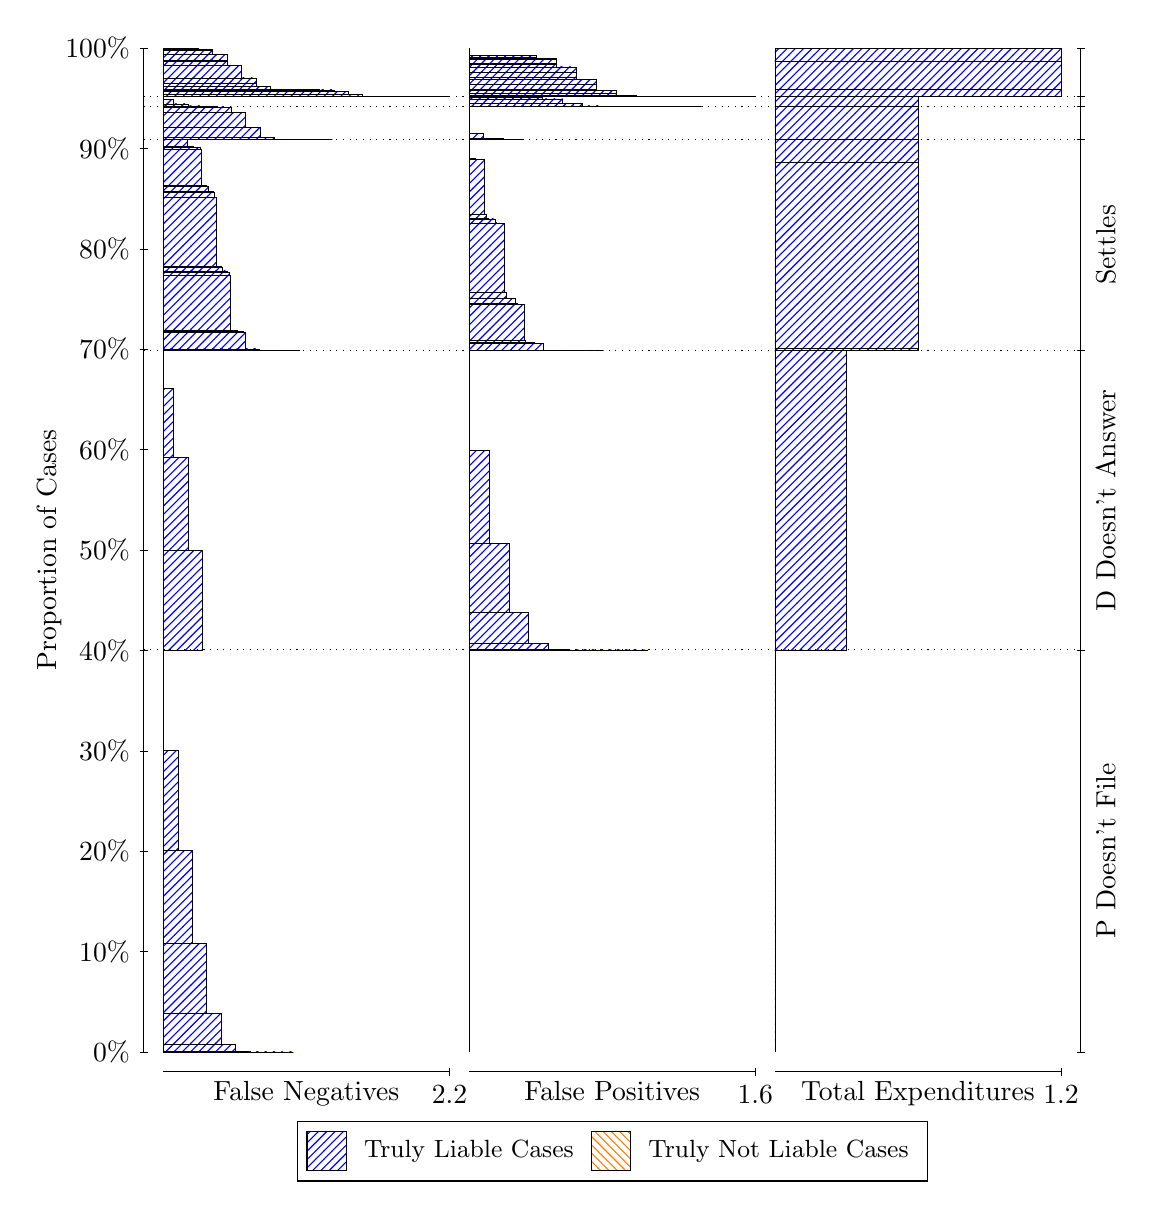
\begin{tikzpicture}
\draw[black, very thin] (1.5,1.75) -- (1.5,14.5);
\node[rotate=90, anchor=center] at (0.3, 8.125) {Proportion of Cases};
\draw[black, very thin] (1.45,1.75) -- (1.55,1.75);
\node[anchor=east] at (1.45, 1.75) {0\%};
\draw[black, very thin] (1.45,3.025) -- (1.55,3.025);
\node[anchor=east] at (1.45, 3.025) {10\%};
\draw[black, very thin] (1.45,4.3) -- (1.55,4.3);
\node[anchor=east] at (1.45, 4.3) {20\%};
\draw[black, very thin] (1.45,5.575) -- (1.55,5.575);
\node[anchor=east] at (1.45, 5.575) {30\%};
\draw[black, very thin] (1.45,6.85) -- (1.55,6.85);
\node[anchor=east] at (1.45, 6.85) {40\%};
\draw[black, very thin] (1.45,8.125) -- (1.55,8.125);
\node[anchor=east] at (1.45, 8.125) {50\%};
\draw[black, very thin] (1.45,9.4) -- (1.55,9.4);
\node[anchor=east] at (1.45, 9.4) {60\%};
\draw[black, very thin] (1.45,10.675) -- (1.55,10.675);
\node[anchor=east] at (1.45, 10.675) {70\%};
\draw[black, very thin] (1.45,11.95) -- (1.55,11.95);
\node[anchor=east] at (1.45, 11.95) {80\%};
\draw[black, very thin] (1.45,13.225) -- (1.55,13.225);
\node[anchor=east] at (1.45, 13.225) {90\%};
\draw[black, very thin] (1.45,14.5) -- (1.55,14.5);
\node[anchor=east] at (1.45, 14.5) {100\%};

\draw[black, very thin] (13.4,1.75) -- (13.4,14.5);
\draw[black, very thin] (13.35,1.75) -- (13.45,1.75);
\node[anchor=west] at (13.35, 1.75) {};
\draw[black, very thin] (13.35,6.8558) -- (13.45,6.8558);
\node[anchor=west] at (13.35, 6.8558) {};
\draw[black, very thin] (13.35,10.658) -- (13.45,10.658);
\node[anchor=west] at (13.35, 10.658) {};
\draw[black, very thin] (13.35,13.342) -- (13.45,13.342);
\node[anchor=west] at (13.35, 13.342) {};
\draw[black, very thin] (13.35,13.761) -- (13.45,13.761);
\node[anchor=west] at (13.35, 13.761) {};
\draw[black, very thin] (13.35,13.881) -- (13.45,13.881);
\node[anchor=west] at (13.35, 13.881) {};
\draw[black, very thin] (13.35,14.5) -- (13.45,14.5);
\node[anchor=west] at (13.35, 14.5) {};

\draw[black, very thin, pattern color=blue, pattern=north east lines] (1.75,1.75) rectangle (3.4015,1.75);
\draw[black, very thin, pattern color=blue, pattern=north east lines] (1.75,1.75) rectangle (3.218,1.75);
\draw[black, very thin, pattern color=blue, pattern=north east lines] (1.75,1.75) rectangle (3.0345,1.7503);
\draw[black, very thin, pattern color=blue, pattern=north east lines] (1.75,1.7503) rectangle (2.851,1.7587);
\draw[black, very thin, pattern color=blue, pattern=north east lines] (1.75,1.7587) rectangle (2.6675,1.8456);
\draw[black, very thin, pattern color=blue, pattern=north east lines] (1.75,1.8456) rectangle (2.484,2.2417);
\draw[black, very thin, pattern color=blue, pattern=north east lines] (1.75,2.2417) rectangle (2.3005,3.1249);
\draw[black, very thin, pattern color=blue, pattern=north east lines] (1.75,3.1249) rectangle (2.117,4.3146);
\draw[black, very thin, pattern color=blue, pattern=north east lines] (1.75,4.3146) rectangle (1.9335,5.5812);
\draw[black, very thin, pattern color=orange, pattern=north west lines] (1.75,5.5812) rectangle (1.75,5.5812);
\draw[black, very thin, pattern color=blue, pattern=north east lines] (1.75,5.5812) rectangle (1.75,6.8558);
\draw[black, very thin, pattern color=blue, pattern=north east lines] (1.75,6.8558) rectangle (2.2455,8.1193);
\draw[black, very thin, pattern color=blue, pattern=north east lines] (1.75,8.1193) rectangle (2.062,9.3031);
\draw[black, very thin, pattern color=blue, pattern=north east lines] (1.75,9.3031) rectangle (1.8785,10.182);
\draw[black, very thin, pattern color=orange, pattern=north west lines] (1.75,10.182) rectangle (1.75,10.182);
\draw[black, very thin, pattern color=blue, pattern=north east lines] (1.75,10.182) rectangle (1.75,10.658);
\draw[black, very thin, pattern color=blue, pattern=north east lines] (1.75,10.658) rectangle (3.4841,10.658);
\draw[black, very thin, pattern color=blue, pattern=north east lines] (1.75,10.658) rectangle (3.4015,10.658);
\draw[black, very thin, pattern color=blue, pattern=north east lines] (1.75,10.658) rectangle (3.3189,10.658);
\draw[black, very thin, pattern color=blue, pattern=north east lines] (1.75,10.658) rectangle (3.3006,10.658);
\draw[black, very thin, pattern color=blue, pattern=north east lines] (1.75,10.658) rectangle (3.2364,10.658);
\draw[black, very thin, pattern color=blue, pattern=north east lines] (1.75,10.658) rectangle (3.218,10.658);
\draw[black, very thin, pattern color=blue, pattern=north east lines] (1.75,10.658) rectangle (3.1538,10.658);
\draw[black, very thin, pattern color=blue, pattern=north east lines] (1.75,10.658) rectangle (3.1354,10.658);
\draw[black, very thin, pattern color=blue, pattern=north east lines] (1.75,10.658) rectangle (3.1171,10.658);
\draw[black, very thin, pattern color=blue, pattern=north east lines] (1.75,10.658) rectangle (3.0529,10.658);
\draw[black, very thin, pattern color=blue, pattern=north east lines] (1.75,10.658) rectangle (3.0345,10.658);
\draw[black, very thin, pattern color=blue, pattern=north east lines] (1.75,10.658) rectangle (2.9703,10.678);
\draw[black, very thin, pattern color=blue, pattern=north east lines] (1.75,10.678) rectangle (2.9519,10.679);
\draw[black, very thin, pattern color=blue, pattern=north east lines] (1.75,10.679) rectangle (2.9336,10.679);
\draw[black, very thin, pattern color=blue, pattern=north east lines] (1.75,10.679) rectangle (2.8694,10.679);
\draw[black, very thin, pattern color=blue, pattern=north east lines] (1.75,10.679) rectangle (2.851,10.679);
\draw[black, very thin, pattern color=blue, pattern=north east lines] (1.75,10.679) rectangle (2.7868,10.888);
\draw[black, very thin, pattern color=blue, pattern=north east lines] (1.75,10.888) rectangle (2.7684,10.898);
\draw[black, very thin, pattern color=blue, pattern=north east lines] (1.75,10.898) rectangle (2.7501,10.9);
\draw[black, very thin, pattern color=blue, pattern=north east lines] (1.75,10.9) rectangle (2.6859,10.91);
\draw[black, very thin, pattern color=blue, pattern=north east lines] (1.75,10.91) rectangle (2.6675,10.912);
\draw[black, very thin, pattern color=blue, pattern=north east lines] (1.75,10.912) rectangle (2.6033,11.608);
\draw[black, very thin, pattern color=blue, pattern=north east lines] (1.75,11.608) rectangle (2.5849,11.656);
\draw[black, very thin, pattern color=blue, pattern=north east lines] (1.75,11.656) rectangle (2.5666,11.669);
\draw[black, very thin, pattern color=blue, pattern=north east lines] (1.75,11.669) rectangle (2.5024,11.72);
\draw[black, very thin, pattern color=blue, pattern=north east lines] (1.75,11.72) rectangle (2.484,11.728);
\draw[black, very thin, pattern color=blue, pattern=north east lines] (1.75,11.728) rectangle (2.4198,12.605);
\draw[black, very thin, pattern color=blue, pattern=north east lines] (1.75,12.605) rectangle (2.4014,12.671);
\draw[black, very thin, pattern color=blue, pattern=north east lines] (1.75,12.671) rectangle (2.3831,12.684);
\draw[black, very thin, pattern color=blue, pattern=north east lines] (1.75,12.684) rectangle (2.3189,12.747);
\draw[black, very thin, pattern color=blue, pattern=north east lines] (1.75,12.747) rectangle (2.3005,12.754);
\draw[black, very thin, pattern color=blue, pattern=north east lines] (1.75,12.754) rectangle (2.2363,13.211);
\draw[black, very thin, pattern color=blue, pattern=north east lines] (1.75,13.211) rectangle (2.2179,13.234);
\draw[black, very thin, pattern color=blue, pattern=north east lines] (1.75,13.234) rectangle (2.1996,13.236);
\draw[black, very thin, pattern color=blue, pattern=north east lines] (1.75,13.236) rectangle (2.1354,13.254);
\draw[black, very thin, pattern color=blue, pattern=north east lines] (1.75,13.254) rectangle (2.117,13.255);
\draw[black, very thin, pattern color=blue, pattern=north east lines] (1.75,13.255) rectangle (2.0528,13.335);
\draw[black, very thin, pattern color=blue, pattern=north east lines] (1.75,13.335) rectangle (2.0344,13.337);
\draw[black, very thin, pattern color=blue, pattern=north east lines] (1.75,13.337) rectangle (2.0161,13.338);
\draw[black, very thin, pattern color=blue, pattern=north east lines] (1.75,13.338) rectangle (1.9519,13.338);
\draw[black, very thin, pattern color=blue, pattern=north east lines] (1.75,13.338) rectangle (1.9335,13.338);
\draw[black, very thin, pattern color=blue, pattern=north east lines] (1.75,13.338) rectangle (1.8693,13.342);
\draw[black, very thin, pattern color=blue, pattern=north east lines] (1.75,13.342) rectangle (1.8509,13.342);
\draw[black, very thin, pattern color=blue, pattern=north east lines] (1.75,13.342) rectangle (1.8326,13.342);
\draw[black, very thin, pattern color=blue, pattern=north east lines] (1.75,13.342) rectangle (1.7684,13.342);
\draw[black, very thin, pattern color=orange, pattern=north west lines] (1.75,13.342) rectangle (1.75,13.342);
\draw[black, very thin, pattern color=blue, pattern=north east lines] (1.75,13.342) rectangle (1.75,13.342);
\draw[black, very thin, pattern color=blue, pattern=north east lines] (1.75,13.342) rectangle (3.897,13.342);
\draw[black, very thin, pattern color=blue, pattern=north east lines] (1.75,13.342) rectangle (3.7135,13.342);
\draw[black, very thin, pattern color=blue, pattern=north east lines] (1.75,13.342) rectangle (3.53,13.342);
\draw[black, very thin, pattern color=blue, pattern=north east lines] (1.75,13.342) rectangle (3.3465,13.343);
\draw[black, very thin, pattern color=blue, pattern=north east lines] (1.75,13.343) rectangle (3.163,13.362);
\draw[black, very thin, pattern color=blue, pattern=north east lines] (1.75,13.362) rectangle (2.9795,13.495);
\draw[black, very thin, pattern color=blue, pattern=north east lines] (1.75,13.495) rectangle (2.796,13.685);
\draw[black, very thin, pattern color=blue, pattern=north east lines] (1.75,13.685) rectangle (2.6125,13.753);
\draw[black, very thin, pattern color=blue, pattern=north east lines] (1.75,13.753) rectangle (2.429,13.761);
\draw[black, very thin, pattern color=blue, pattern=north east lines] (1.75,13.761) rectangle (2.2455,13.761);
\draw[black, very thin, pattern color=orange, pattern=north west lines] (1.75,13.761) rectangle (1.75,13.761);
\draw[black, very thin, pattern color=blue, pattern=north east lines] (1.75,13.761) rectangle (2.2455,13.765);
\draw[black, very thin, pattern color=blue, pattern=north east lines] (1.75,13.765) rectangle (2.062,13.79);
\draw[black, very thin, pattern color=blue, pattern=north east lines] (1.75,13.79) rectangle (1.8785,13.846);
\draw[black, very thin, pattern color=orange, pattern=north west lines] (1.75,13.846) rectangle (1.75,13.846);
\draw[black, very thin, pattern color=blue, pattern=north east lines] (1.75,13.846) rectangle (1.75,13.881);
\draw[black, very thin, pattern color=blue, pattern=north east lines] (1.75,13.881) rectangle (5.3833,13.881);
\draw[black, very thin, pattern color=blue, pattern=north east lines] (1.75,13.881) rectangle (5.1998,13.881);
\draw[black, very thin, pattern color=blue, pattern=north east lines] (1.75,13.881) rectangle (5.0163,13.881);
\draw[black, very thin, pattern color=blue, pattern=north east lines] (1.75,13.881) rectangle (5.0163,13.881);
\draw[black, very thin, pattern color=blue, pattern=north east lines] (1.75,13.881) rectangle (4.8328,13.881);
\draw[black, very thin, pattern color=blue, pattern=north east lines] (1.75,13.881) rectangle (4.6493,13.882);
\draw[black, very thin, pattern color=blue, pattern=north east lines] (1.75,13.882) rectangle (4.4658,13.887);
\draw[black, very thin, pattern color=blue, pattern=north east lines] (1.75,13.887) rectangle (4.2823,13.908);
\draw[black, very thin, pattern color=blue, pattern=north east lines] (1.75,13.908) rectangle (4.0988,13.914);
\draw[black, very thin, pattern color=blue, pattern=north east lines] (1.75,13.914) rectangle (4.0988,13.946);
\draw[black, very thin, pattern color=blue, pattern=north east lines] (1.75,13.946) rectangle (4.0254,13.946);
\draw[black, very thin, pattern color=blue, pattern=north east lines] (1.75,13.946) rectangle (3.9153,13.968);
\draw[black, very thin, pattern color=blue, pattern=north east lines] (1.75,13.968) rectangle (3.9153,13.969);
\draw[black, very thin, pattern color=blue, pattern=north east lines] (1.75,13.969) rectangle (3.8419,13.969);
\draw[black, very thin, pattern color=blue, pattern=north east lines] (1.75,13.969) rectangle (3.7318,13.973);
\draw[black, very thin, pattern color=blue, pattern=north east lines] (1.75,13.973) rectangle (3.6584,13.973);
\draw[black, very thin, pattern color=blue, pattern=north east lines] (1.75,13.973) rectangle (3.5483,13.974);
\draw[black, very thin, pattern color=blue, pattern=north east lines] (1.75,13.974) rectangle (3.5483,13.974);
\draw[black, very thin, pattern color=blue, pattern=north east lines] (1.75,13.974) rectangle (3.4749,13.974);
\draw[black, very thin, pattern color=blue, pattern=north east lines] (1.75,13.974) rectangle (3.4749,13.974);
\draw[black, very thin, pattern color=blue, pattern=north east lines] (1.75,13.974) rectangle (3.3648,13.974);
\draw[black, very thin, pattern color=blue, pattern=north east lines] (1.75,13.974) rectangle (3.3648,13.974);
\draw[black, very thin, pattern color=blue, pattern=north east lines] (1.75,13.974) rectangle (3.2914,13.975);
\draw[black, very thin, pattern color=blue, pattern=north east lines] (1.75,13.975) rectangle (3.2914,13.977);
\draw[black, very thin, pattern color=blue, pattern=north east lines] (1.75,13.977) rectangle (3.1813,13.977);
\draw[black, very thin, pattern color=blue, pattern=north east lines] (1.75,13.977) rectangle (3.1079,14.009);
\draw[black, very thin, pattern color=blue, pattern=north east lines] (1.75,14.009) rectangle (2.9978,14.009);
\draw[black, very thin, pattern color=blue, pattern=north east lines] (1.75,14.009) rectangle (2.9244,14.056);
\draw[black, very thin, pattern color=blue, pattern=north east lines] (1.75,14.056) rectangle (2.9244,14.121);
\draw[black, very thin, pattern color=blue, pattern=north east lines] (1.75,14.121) rectangle (2.7409,14.284);
\draw[black, very thin, pattern color=blue, pattern=north east lines] (1.75,14.284) rectangle (2.5574,14.335);
\draw[black, very thin, pattern color=blue, pattern=north east lines] (1.75,14.335) rectangle (2.5574,14.35);
\draw[black, very thin, pattern color=blue, pattern=north east lines] (1.75,14.35) rectangle (2.5574,14.417);
\draw[black, very thin, pattern color=blue, pattern=north east lines] (1.75,14.417) rectangle (2.3739,14.474);
\draw[black, very thin, pattern color=blue, pattern=north east lines] (1.75,14.474) rectangle (2.3739,14.481);
\draw[black, very thin, pattern color=blue, pattern=north east lines] (1.75,14.481) rectangle (2.1904,14.484);
\draw[black, very thin, pattern color=blue, pattern=north east lines] (1.75,14.484) rectangle (2.1904,14.487);
\draw[black, very thin, pattern color=blue, pattern=north east lines] (1.75,14.487) rectangle (2.1904,14.497);
\draw[black, very thin, pattern color=blue, pattern=north east lines] (1.75,14.497) rectangle (2.0069,14.499);
\draw[black, very thin, pattern color=blue, pattern=north east lines] (1.75,14.499) rectangle (2.0069,14.5);
\draw[black, very thin, pattern color=blue, pattern=north east lines] (1.75,14.5) rectangle (1.8234,14.5);
\draw[black, very thin, pattern color=blue, pattern=north east lines] (1.75,14.5) rectangle (1.8234,14.5);
\draw[black, very thin, pattern color=orange, pattern=north west lines] (1.75,14.5) rectangle (1.75,14.5);
\draw[black, very thin, pattern color=blue, pattern=north east lines] (1.75,14.5) rectangle (1.75,14.5);
\draw[black, very thin, pattern color=orange, pattern=north west lines] (5.6333,1.75) rectangle (5.6333,1.75);
\draw[black, very thin, pattern color=blue, pattern=north east lines] (5.6333,1.75) rectangle (5.6333,6.8558);
\draw[black, very thin, pattern color=orange, pattern=north west lines] (5.6333,6.8558) rectangle (7.9042,6.8558);
\draw[black, very thin, pattern color=blue, pattern=north east lines] (5.6333,6.8558) rectangle (7.9042,6.8558);
\draw[black, very thin, pattern color=blue, pattern=north east lines] (5.6333,6.8558) rectangle (7.6519,6.8558);
\draw[black, very thin, pattern color=blue, pattern=north east lines] (5.6333,6.8558) rectangle (7.3995,6.8558);
\draw[black, very thin, pattern color=blue, pattern=north east lines] (5.6333,6.8558) rectangle (7.1472,6.8559);
\draw[black, very thin, pattern color=blue, pattern=north east lines] (5.6333,6.8559) rectangle (6.8949,6.8613);
\draw[black, very thin, pattern color=blue, pattern=north east lines] (5.6333,6.8613) rectangle (6.6426,6.9407);
\draw[black, very thin, pattern color=blue, pattern=north east lines] (5.6333,6.9407) rectangle (6.3903,7.3313);
\draw[black, very thin, pattern color=blue, pattern=north east lines] (5.6333,7.3313) rectangle (6.138,8.2102);
\draw[black, very thin, pattern color=blue, pattern=north east lines] (5.6333,8.2102) rectangle (5.8856,9.3939);
\draw[black, very thin, pattern color=blue, pattern=north east lines] (5.6333,9.3939) rectangle (5.6333,10.658);
\draw[black, very thin, pattern color=orange, pattern=north west lines] (5.6333,10.658) rectangle (7.3365,10.658);
\draw[black, very thin, pattern color=blue, pattern=north east lines] (5.6333,10.658) rectangle (7.3365,10.658);
\draw[black, very thin, pattern color=orange, pattern=north west lines] (5.6333,10.658) rectangle (7.2229,10.658);
\draw[black, very thin, pattern color=blue, pattern=north east lines] (5.6333,10.658) rectangle (7.2229,10.658);
\draw[black, very thin, pattern color=orange, pattern=north west lines] (5.6333,10.658) rectangle (7.1094,10.658);
\draw[black, very thin, pattern color=blue, pattern=north east lines] (5.6333,10.658) rectangle (7.1094,10.658);
\draw[black, very thin, pattern color=blue, pattern=north east lines] (5.6333,10.658) rectangle (7.0841,10.658);
\draw[black, very thin, pattern color=orange, pattern=north west lines] (5.6333,10.658) rectangle (6.9958,10.658);
\draw[black, very thin, pattern color=blue, pattern=north east lines] (5.6333,10.658) rectangle (6.9958,10.658);
\draw[black, very thin, pattern color=blue, pattern=north east lines] (5.6333,10.658) rectangle (6.9706,10.658);
\draw[black, very thin, pattern color=orange, pattern=north west lines] (5.6333,10.658) rectangle (6.8823,10.658);
\draw[black, very thin, pattern color=blue, pattern=north east lines] (5.6333,10.658) rectangle (6.8823,10.658);
\draw[black, very thin, pattern color=blue, pattern=north east lines] (5.6333,10.658) rectangle (6.8571,10.658);
\draw[black, very thin, pattern color=blue, pattern=north east lines] (5.6333,10.658) rectangle (6.8318,10.661);
\draw[black, very thin, pattern color=blue, pattern=north east lines] (5.6333,10.661) rectangle (6.7435,10.661);
\draw[black, very thin, pattern color=blue, pattern=north east lines] (5.6333,10.661) rectangle (6.7183,10.662);
\draw[black, very thin, pattern color=blue, pattern=north east lines] (5.6333,10.662) rectangle (6.63,10.662);
\draw[black, very thin, pattern color=blue, pattern=north east lines] (5.6333,10.662) rectangle (6.6047,10.664);
\draw[black, very thin, pattern color=blue, pattern=north east lines] (5.6333,10.664) rectangle (6.5795,10.745);
\draw[black, very thin, pattern color=blue, pattern=north east lines] (5.6333,10.745) rectangle (6.4912,10.746);
\draw[black, very thin, pattern color=blue, pattern=north east lines] (5.6333,10.746) rectangle (6.466,10.764);
\draw[black, very thin, pattern color=blue, pattern=north east lines] (5.6333,10.764) rectangle (6.3777,10.766);
\draw[black, very thin, pattern color=blue, pattern=north east lines] (5.6333,10.766) rectangle (6.3524,10.789);
\draw[black, very thin, pattern color=blue, pattern=north east lines] (5.6333,10.789) rectangle (6.3272,11.246);
\draw[black, very thin, pattern color=blue, pattern=north east lines] (5.6333,11.246) rectangle (6.2389,11.253);
\draw[black, very thin, pattern color=blue, pattern=north east lines] (5.6333,11.253) rectangle (6.2137,11.316);
\draw[black, very thin, pattern color=blue, pattern=north east lines] (5.6333,11.316) rectangle (6.1253,11.328);
\draw[black, very thin, pattern color=blue, pattern=north east lines] (5.6333,11.328) rectangle (6.1001,11.394);
\draw[black, very thin, pattern color=blue, pattern=north east lines] (5.6333,11.394) rectangle (6.0749,12.271);
\draw[black, very thin, pattern color=blue, pattern=north east lines] (5.6333,12.271) rectangle (5.9866,12.28);
\draw[black, very thin, pattern color=blue, pattern=north east lines] (5.6333,12.28) rectangle (5.9613,12.331);
\draw[black, very thin, pattern color=blue, pattern=north east lines] (5.6333,12.331) rectangle (5.873,12.344);
\draw[black, very thin, pattern color=blue, pattern=north east lines] (5.6333,12.344) rectangle (5.8478,12.392);
\draw[black, very thin, pattern color=blue, pattern=north east lines] (5.6333,12.392) rectangle (5.8226,13.088);
\draw[black, very thin, pattern color=blue, pattern=north east lines] (5.6333,13.088) rectangle (5.7343,13.09);
\draw[black, very thin, pattern color=blue, pattern=north east lines] (5.6333,13.09) rectangle (5.709,13.1);
\draw[black, very thin, pattern color=blue, pattern=north east lines] (5.6333,13.1) rectangle (5.6333,13.342);
\draw[black, very thin, pattern color=orange, pattern=north west lines] (5.6333,13.342) rectangle (6.3146,13.342);
\draw[black, very thin, pattern color=blue, pattern=north east lines] (5.6333,13.342) rectangle (6.3146,13.343);
\draw[black, very thin, pattern color=blue, pattern=north east lines] (5.6333,13.343) rectangle (6.0623,13.351);
\draw[black, very thin, pattern color=blue, pattern=north east lines] (5.6333,13.351) rectangle (5.81,13.419);
\draw[black, very thin, pattern color=blue, pattern=north east lines] (5.6333,13.419) rectangle (5.6333,13.761);
\draw[black, very thin, pattern color=orange, pattern=north west lines] (5.6333,13.761) rectangle (8.5854,13.761);
\draw[black, very thin, pattern color=blue, pattern=north east lines] (5.6333,13.761) rectangle (8.5854,13.761);
\draw[black, very thin, pattern color=blue, pattern=north east lines] (5.6333,13.761) rectangle (8.3331,13.761);
\draw[black, very thin, pattern color=blue, pattern=north east lines] (5.6333,13.761) rectangle (8.0808,13.761);
\draw[black, very thin, pattern color=blue, pattern=north east lines] (5.6333,13.761) rectangle (7.8285,13.761);
\draw[black, very thin, pattern color=blue, pattern=north east lines] (5.6333,13.761) rectangle (7.5762,13.761);
\draw[black, very thin, pattern color=blue, pattern=north east lines] (5.6333,13.761) rectangle (7.3238,13.765);
\draw[black, very thin, pattern color=blue, pattern=north east lines] (5.6333,13.765) rectangle (7.0715,13.797);
\draw[black, very thin, pattern color=blue, pattern=north east lines] (5.6333,13.797) rectangle (6.8192,13.853);
\draw[black, very thin, pattern color=blue, pattern=north east lines] (5.6333,13.853) rectangle (6.5669,13.877);
\draw[black, very thin, pattern color=blue, pattern=north east lines] (5.6333,13.877) rectangle (6.3146,13.881);
\draw[black, very thin, pattern color=orange, pattern=north west lines] (5.6333,13.881) rectangle (9.2667,13.881);
\draw[black, very thin, pattern color=blue, pattern=north east lines] (5.6333,13.881) rectangle (9.2667,13.881);
\draw[black, very thin, pattern color=orange, pattern=north west lines] (5.6333,13.881) rectangle (9.0144,13.881);
\draw[black, very thin, pattern color=blue, pattern=north east lines] (5.6333,13.881) rectangle (9.0144,13.881);
\draw[black, very thin, pattern color=orange, pattern=north west lines] (5.6333,13.881) rectangle (8.762,13.881);
\draw[black, very thin, pattern color=blue, pattern=north east lines] (5.6333,13.881) rectangle (8.762,13.881);
\draw[black, very thin, pattern color=blue, pattern=north east lines] (5.6333,13.881) rectangle (8.5097,13.881);
\draw[black, very thin, pattern color=orange, pattern=north west lines] (5.6333,13.881) rectangle (8.5097,13.881);
\draw[black, very thin, pattern color=blue, pattern=north east lines] (5.6333,13.881) rectangle (8.5097,13.881);
\draw[black, very thin, pattern color=blue, pattern=north east lines] (5.6333,13.881) rectangle (8.2574,13.882);
\draw[black, very thin, pattern color=orange, pattern=north west lines] (5.6333,13.882) rectangle (8.2574,13.882);
\draw[black, very thin, pattern color=blue, pattern=north east lines] (5.6333,13.882) rectangle (8.2574,13.882);
\draw[black, very thin, pattern color=blue, pattern=north east lines] (5.6333,13.882) rectangle (8.0051,13.884);
\draw[black, very thin, pattern color=orange, pattern=north west lines] (5.6333,13.884) rectangle (8.0051,13.884);
\draw[black, very thin, pattern color=blue, pattern=north east lines] (5.6333,13.884) rectangle (8.0051,13.884);
\draw[black, very thin, pattern color=blue, pattern=north east lines] (5.6333,13.884) rectangle (7.7528,13.889);
\draw[black, very thin, pattern color=orange, pattern=north west lines] (5.6333,13.889) rectangle (7.7528,13.889);
\draw[black, very thin, pattern color=blue, pattern=north east lines] (5.6333,13.889) rectangle (7.7528,13.901);
\draw[black, very thin, pattern color=blue, pattern=north east lines] (5.6333,13.901) rectangle (7.7528,13.901);
\draw[black, very thin, pattern color=blue, pattern=north east lines] (5.6333,13.901) rectangle (7.7528,13.901);
\draw[black, very thin, pattern color=blue, pattern=north east lines] (5.6333,13.901) rectangle (7.5005,13.93);
\draw[black, very thin, pattern color=orange, pattern=north west lines] (5.6333,13.93) rectangle (7.5005,13.93);
\draw[black, very thin, pattern color=blue, pattern=north east lines] (5.6333,13.93) rectangle (7.5005,13.964);
\draw[black, very thin, pattern color=blue, pattern=north east lines] (5.6333,13.964) rectangle (7.5005,13.965);
\draw[black, very thin, pattern color=blue, pattern=north east lines] (5.6333,13.965) rectangle (7.2481,13.976);
\draw[black, very thin, pattern color=blue, pattern=north east lines] (5.6333,13.976) rectangle (7.2481,14.034);
\draw[black, very thin, pattern color=blue, pattern=north east lines] (5.6333,14.034) rectangle (7.2481,14.097);
\draw[black, very thin, pattern color=blue, pattern=north east lines] (5.6333,14.097) rectangle (6.9958,14.127);
\draw[black, very thin, pattern color=blue, pattern=north east lines] (5.6333,14.127) rectangle (6.9958,14.198);
\draw[black, very thin, pattern color=blue, pattern=north east lines] (5.6333,14.198) rectangle (6.9958,14.26);
\draw[black, very thin, pattern color=blue, pattern=north east lines] (5.6333,14.26) rectangle (6.7435,14.294);
\draw[black, very thin, pattern color=blue, pattern=north east lines] (5.6333,14.294) rectangle (6.7435,14.3);
\draw[black, very thin, pattern color=blue, pattern=north east lines] (5.6333,14.3) rectangle (6.7435,14.356);
\draw[black, very thin, pattern color=blue, pattern=north east lines] (5.6333,14.356) rectangle (6.7435,14.372);
\draw[black, very thin, pattern color=orange, pattern=north west lines] (5.6333,14.372) rectangle (6.6426,14.372);
\draw[black, very thin, pattern color=blue, pattern=north east lines] (5.6333,14.372) rectangle (6.6426,14.372);
\draw[black, very thin, pattern color=blue, pattern=north east lines] (5.6333,14.372) rectangle (6.4912,14.388);
\draw[black, very thin, pattern color=blue, pattern=north east lines] (5.6333,14.388) rectangle (6.4912,14.405);
\draw[black, very thin, pattern color=orange, pattern=north west lines] (5.6333,14.405) rectangle (6.3903,14.405);
\draw[black, very thin, pattern color=blue, pattern=north east lines] (5.6333,14.405) rectangle (6.3903,14.405);
\draw[black, very thin, pattern color=blue, pattern=north east lines] (5.6333,14.405) rectangle (6.2389,14.405);
\draw[black, very thin, pattern color=blue, pattern=north east lines] (5.6333,14.405) rectangle (6.2389,14.408);
\draw[black, very thin, pattern color=blue, pattern=north east lines] (5.6333,14.408) rectangle (6.2389,14.408);
\draw[black, very thin, pattern color=orange, pattern=north west lines] (5.6333,14.408) rectangle (6.138,14.408);
\draw[black, very thin, pattern color=blue, pattern=north east lines] (5.6333,14.408) rectangle (6.138,14.408);
\draw[black, very thin, pattern color=blue, pattern=north east lines] (5.6333,14.408) rectangle (5.9866,14.408);
\draw[black, very thin, pattern color=blue, pattern=north east lines] (5.6333,14.408) rectangle (5.9866,14.408);
\draw[black, very thin, pattern color=orange, pattern=north west lines] (5.6333,14.408) rectangle (5.8856,14.408);
\draw[black, very thin, pattern color=blue, pattern=north east lines] (5.6333,14.408) rectangle (5.8856,14.408);
\draw[black, very thin, pattern color=blue, pattern=north east lines] (5.6333,14.408) rectangle (5.7343,14.408);
\draw[black, very thin, pattern color=blue, pattern=north east lines] (5.6333,14.408) rectangle (5.7343,14.408);
\draw[black, very thin, pattern color=blue, pattern=north east lines] (5.6333,14.408) rectangle (5.7343,14.408);
\draw[black, very thin, pattern color=orange, pattern=north west lines] (5.6333,14.408) rectangle (5.6333,14.408);
\draw[black, very thin, pattern color=blue, pattern=north east lines] (5.6333,14.408) rectangle (5.6333,14.5);
\draw[black, very thin, pattern color=orange, pattern=north west lines] (9.5167,1.75) rectangle (9.5167,1.75);
\draw[black, very thin, pattern color=blue, pattern=north east lines] (9.5167,1.75) rectangle (9.5167,6.8558);
\draw[black, very thin, pattern color=orange, pattern=north west lines] (9.5167,6.8558) rectangle (10.425,6.8558);
\draw[black, very thin, pattern color=blue, pattern=north east lines] (9.5167,6.8558) rectangle (10.425,10.658);
\draw[black, very thin, pattern color=orange, pattern=north west lines] (9.5167,10.658) rectangle (11.333,10.658);
\draw[black, very thin, pattern color=blue, pattern=north east lines] (9.5167,10.658) rectangle (11.333,10.687);
\draw[black, very thin, pattern color=orange, pattern=north west lines] (9.5167,10.687) rectangle (11.333,10.687);
\draw[black, very thin, pattern color=blue, pattern=north east lines] (9.5167,10.687) rectangle (11.333,13.05);
\draw[black, very thin, pattern color=orange, pattern=north west lines] (9.5167,13.05) rectangle (11.333,13.05);
\draw[black, very thin, pattern color=blue, pattern=north east lines] (9.5167,13.05) rectangle (11.333,13.342);
\draw[black, very thin, pattern color=orange, pattern=north west lines] (9.5167,13.342) rectangle (11.333,13.342);
\draw[black, very thin, pattern color=blue, pattern=north east lines] (9.5167,13.342) rectangle (11.333,13.761);
\draw[black, very thin, pattern color=orange, pattern=north west lines] (9.5167,13.761) rectangle (11.333,13.761);
\draw[black, very thin, pattern color=blue, pattern=north east lines] (9.5167,13.761) rectangle (11.333,13.881);
\draw[black, very thin, pattern color=orange, pattern=north west lines] (9.5167,13.881) rectangle (13.15,13.881);
\draw[black, very thin, pattern color=blue, pattern=north east lines] (9.5167,13.881) rectangle (13.15,13.982);
\draw[black, very thin, pattern color=orange, pattern=north west lines] (9.5167,13.982) rectangle (13.15,13.982);
\draw[black, very thin, pattern color=blue, pattern=north east lines] (9.5167,13.982) rectangle (13.15,14.327);
\draw[black, very thin, pattern color=orange, pattern=north west lines] (9.5167,14.327) rectangle (13.15,14.327);
\draw[black, very thin, pattern color=blue, pattern=north east lines] (9.5167,14.327) rectangle (13.15,14.5);
\draw[black, dotted] (1.5,6.8558) -- (13.4,6.8558);
\draw[black, dotted] (1.5,10.658) -- (13.4,10.658);
\draw[black, dotted] (1.5,13.342) -- (13.4,13.342);
\draw[black, dotted] (1.5,13.761) -- (13.4,13.761);
\draw[black, dotted] (1.5,13.881) -- (13.4,13.881);
\draw[black, very thin] (1.75,1.5) -- (5.3833,1.5);
\node[anchor=north] at (3.5667, 1.5) {False Negatives};
\draw[black, very thin] (5.3833,1.45) -- (5.3833,1.55);
\node[anchor=north] at (5.3833, 1.45) {2.2};

\draw[black, very thin] (5.6333,1.5) -- (9.2667,1.5);
\node[anchor=north] at (7.45, 1.5) {False Positives};
\draw[black, very thin] (9.2667,1.45) -- (9.2667,1.55);
\node[anchor=north] at (9.2667, 1.45) {1.6};

\draw[black, very thin] (9.5167,1.5) -- (13.15,1.5);
\node[anchor=north] at (11.333, 1.5) {Total Expenditures};
\draw[black, very thin] (13.15,1.45) -- (13.15,1.55);
\node[anchor=north] at (13.15, 1.45) {1.2};

\node[black, centered, rotate=90] at (13.72, 4.3029) {P Doesn't File};
\node[black, centered, rotate=90] at (13.72, 8.7566) {D Doesn't Answer};
\node[black, centered, rotate=90] at (13.72, 12) {Settles};




\draw (7.449999999999999,1.5) node[draw=none] (baseCoordinate) {};
\begin{scope}[align=center]
        \matrix[scale=0.5, draw=black, below=0.5cm of baseCoordinate, nodes={draw}, column sep=0.1cm]{
            \node[rectangle, draw, minimum width=0.5cm, minimum height=0.5cm, pattern=north east lines, pattern color=blue] {}; &
            \node[draw=none, font=\small] (B) {Truly Liable Cases}; &
            \node[rectangle, draw, minimum width=0.5cm, minimum height=0.5cm, pattern=north west lines, pattern color=orange] {}; &
            \node[draw=none, font=\small] (B) {Truly Not Liable Cases}; \\
            };
\end{scope}

\end{tikzpicture}
\end{document}